\documentclass[a4paper, 11pt]{report}

\usepackage{fullpage}



\usepackage[utf8]{inputenc} 
\usepackage[T1]{fontenc}
\usepackage{lmodern}
\usepackage{graphicx}
\usepackage[french]{babel}
\usepackage{color}
%\usepackage{fullpage}
\usepackage{array}
\usepackage[tight]{shorttoc}
\usepackage[toc,page]{appendix} 
\usepackage{makeidx} 
\usepackage{titlesec} % pour enlever "chapitre"


\definecolor{gris}{gray}{0.45}

\newcommand{\rouge}[1]{\textcolor{red}{#1}}
\newcommand{\rem}[1]{\textcolor{blue}{\emph{Remarque: \\} #1}}
\newcommand{\exl}[1]{\textcolor{gris}{\emph{Exemple: } #1}}
\newcommand{\exc}[1]{\textcolor{gris}{(\emph{Ex:} #1)}}
\newcommand{\cod}[1]{\textcolor{gris}{\emph{#1}}} 
\newcommand{\att}[1]{\textcolor{red}{\emph{\\ Attention: \\} #1 \\}}

\usepackage{listings}
\definecolor{dkgreen}{rgb}{0,0.6,0}
\definecolor{gray}{rgb}{0.5,0.5,0.5}
\definecolor{mauve}{rgb}{0.58,0,0.82}
\definecolor{red}{rgb}{1,0,0}

\newcommand{\lstconfig}[1]{
	\lstset{
	  language=#1,				      % the language of the code
	  basicstyle=\footnotesize,	      % the size of the fonts that are used for the code
	  numbers=left,				      % where to put the line-numbers
	  numberstyle=\footnotesize,	  % the size of the fonts that are used for the line-numbers
	  stepnumber=1,				      % the step between two line-numbers. If it's 1, each line 
									  % will be numbered
	  numbersep=5pt,				  % how far the line-numbers are from the code
	  backgroundcolor=\color{white},  % choose the background color. You must add \usepackage{color}
	  showspaces=false,			      % show spaces adding particular underscores
	  showstringspaces=false,		  % underline spaces within strings
	  showtabs=false,				  % show tabs within strings adding particular underscores
	  frame=single,				      % adds a frame around the code
	  tabsize=2,					  % sets default tabsize to 2 spaces
	  captionpos=b,				      % sets the caption-position to bottom
	  breaklines=true,				  % sets automatic line breaking
	  breakatwhitespace=false,		  % sets if automatic breaks should only happen at whitespace
	  title=\lstname,	   			  % show the filename of files included with \lstinputlisting;
									  % also try caption instead of title
	  numberstyle=\tiny\color{gray},  % line number style
	  keywordstyle=\color{blue},	  % keyword style
	  commentstyle=\color{dkgreen}\textit,   % comment style
	  stringstyle=\color{mauve}\textbf,	  % string literal style
	}
}
	
	\titleformat{\chapter}[hang]{\bf\huge}{\thechapter}{2pc}{} 
	\renewcommand{\appendixpagename}{Annexes}  
	\renewcommand{\appendixtocname}{Annexes}    
  

\begin{document}



\makeatletter
	\def\clap#1{\hbox to 0pt{\hss #1\hss}}%
	\def\ligne#1{%
	\hbox to \hsize{%
	\vbox{\centering #1}}}%
	\def\haut#1#2#3{%
	\hbox to \hsize{%
	\rlap{\vtop{\raggedright #1}}%
	\hss
	\clap{\vtop{\centering #2}}%
	\hss
	\llap{\vtop{\raggedleft #3}}}}%
	\def\bas#1#2#3{%
	\hbox to \hsize{%
	\rlap{\vbox{\raggedright #1}}%
	\hss
	\clap{\vbox{\centering #2}}%
	\hss
	\llap{\vbox{\raggedleft #3}}}}%
	\def\maketitle{%
	\thispagestyle{empty}\vbox to \vsize{%
	\haut{}{\@blurb}{}
	\vfill
	\vspace{1cm}
\begin{flushleft}
	%\usefont{OT1}{ptm}{m}{n}
	\huge \@title
\end{flushleft}
	\par
	\hrule height 4pt
	\par
\begin{flushright}
	%\usefont{OT1}{phv}{m}{n}
	\Large \@author
	\par
\end{flushright}
	\vspace{1cm}
	\vfill
	\vfill

\begin{center}
	
\includegraphics[width=5cm]{logo_UTBM.jpg}
\end{center}

\bas{}{Printemps 2013}{}
}%
\cleardoublepage
}
\def\date#1{\def\@date{#1}}
\def\author#1{\def\@author{#1}}
\def\title#1{\def\@title{#1}}
\def\location#1{\def\@location{#1}}
\def\blurb#1{\def\@blurb{#1}}
\date{\today}
\author{}
\title{}

% informations
\location{Belfort}\blurb{}
\makeatother
\title{Projet de résolution d'un tangram}
\author{\small{Adrien \bsc{Berthet}, Paul \bsc{Locatelli} et Pierre \bsc{Rognon}}}
\blurb{%
	\textbf{IA41 - Concepts fondamentaux en Intelligence Artificielle et langages dédiés}\\
	Université de Technologie de Belfort-Montbéliard
}% 


	
	\maketitle
	
	\newpage
	
	\shorttoc{Sommaire}{0}
	
	
	\chapter*{Introduction}
	\addcontentsline{toc}{chapter}{Introduction}
	
		Pour ce projet, le sujet abordant le casse-tête du tangram (numéro 6) a été retenu. Le choix de ce sujet s'est fait sur l'intérêt de ce jeu. En effet, s'il apparaît assez aisé de résoudre des modèles tels que le classique "carré" que chacun connaît, d'autres modèles sont beaucoup plus complexes. De plus, c'est un test utilisé dans de nombreux tests afin de déceler d'éventuelles déficiences chez les enfants tels que le WISC (Wechsler Intelligence Scale for Children). C'est donc un problème d'Intelligence Artificielle fondamental qui sera abordé dans ce projet et dont la résolution sera tentée.\\
L'analyse de ce problème constitue une partie prépondérante dans la tentative de résolution du tangram. Environ 6000 configurations différentes sont connues aujourd'hui. De nombreux modèles ont donc dû être envisagés afin de couvrir l'ensemble des cas possibles. Une seconde phase qui s'avère aussi complexe est le choix des différentes représentations informatiques du problème. De nombreux traitements ont été effectués pour mettre à bien cette partie. Quelques exemples qui ont été utilisés comme support durant toute la durée du projet seront présentés afin d'indiquer leur solution. Enfin, la résolution par le logiciel crée sera abordée pour ces exemples. Les limites de ce problème et l'état d'avancement du projet seront indiqués enfin.


	\newpage

	\chapter{Analyse du casse-t\^ete}
	
	Une première analyse du tangram a permis de mettre à jour plusieurs sous-problèmes. Deux problèmes d'ordre mathématique ainsi qu'un problème d'intelligence artificielle pure ont ainsi été isolés. 
	
		\section{Placement de pièce dans un modèle}
		
		Le premier problème à résoudre est le placement d'une pièce dans un modèle. L'objectif de cette méthode est ainsi de renvoyer l'ensemble des positions possibles pour une pièce dans le modèle.\\
		Pour le développement de cette méthode, l'analyse s'est faite sur la base du raisonnement humain. La première approche, la plus simple pour un humain, consiste à tester toutes les positions possibles que peut prendre une pièce.\\
		Si cette approche par\^ait intéressante et rapide à effectuer par un cerveau humain, du point de vue de la programmation et donc de l'intelligence artificielle, cette méthode n'est pas très efficace, puisqu'elle implique de tester toutes les solutions.\\
		Pour une résolution efficace, après étude de différentes possibilités, il est apparu qu'il était préférable de "coller" les pièces à une arête du modèle. Cependant, ce "matching" doit se faire d'une manière intelligente. \\
		Le but est donc de chercher les points communs entre la pièce et le modèle afin de trouver un point ou une arête constituant la base du placement de la pièce. Le premier point commun possible entre la pièce et le modèle est la longueur d'une arête. En effet, les pièces du Tangram ayant chacune des caractéristiques différentes, si une arête du dessin coïncide avec une arête de la pièce, il y a de grandes chances pour que la pièce soit positionnée à cet endroit. 
    
    \begin{center}
    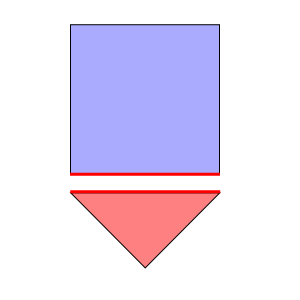
\includegraphics[width=5cm]{place_figure_exacte_match}\\
    \emph{Ici, on peut voir que le triangle a une arête qui coïncide exactement avec une arête du modèle.}\\
    \end{center}

    S'il est évident que cette méthode est efficace dans de nombreux cas, elle a ses limites: il se peut que lors de la résolution du Tangram, une arête du modèle corresponde à plusieurs pièces. Lors de ce type de configurations la première méthode est donc inefficace. 

    \begin{center}
    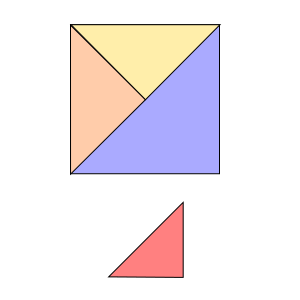
\includegraphics[width=5cm]{place_figure_probleme_exacte_match}\\
    \emph{Un problème peut arriver si plusieurs pièces coïncident avec une arête.}\\
    \end{center}

    Un second point commun, qui va pouvoir résoudre le problème précédent, a été trouvé. Cette seconde caractéristique commune, utile pour la décision de placement de la pièce, est l'utilisation des angles de chaque pièce. Cette méthode n'est utilisée que lorsque la première méthode est inefficace. Il faut alors vérifier si un angle du modèle est égal à l'un des angles de la pièce. 

    \begin{center}
    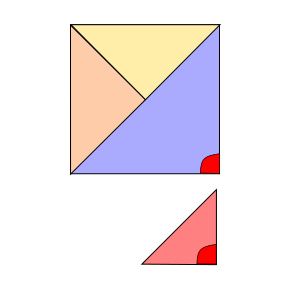
\includegraphics[width=5cm]{place_figure_probleme_angle_match}\\
    \emph{Dans ce cas, on remarque qu'aucune arête ne coïncide. La méthode des angles est donc appliquée et l'on trouve un angle égal.}\\
    \end{center}

    Une fois la base du placement de la pièce trouvée (le point où l'angle correspond entre pièce et modèle), on obtient soit une arête, soit un angle composé de deux arêtes. Il faut ensuite positionner la pièce en fonction de l'arête (ou des arêtes) à l'aide de translation(s) et rotation(s).\\
    Cependant une fois la pièce correctement placée sur le modèle par rapport à la base, un problème important demeure. En effet, selon la rotation et le sens initiale de la pièce, celle-ci peut se trouver à l'inverse de la position voulue. 

    \begin{center}
    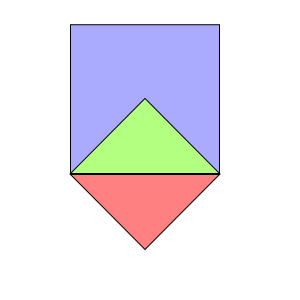
\includegraphics[width=5cm]{place_figure_probleme_symetrie_1}
    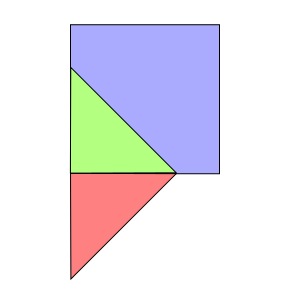
\includegraphics[width=5cm]{place_figure_probleme_symetrie_2}\\
    \emph{Dans les deux figures ci-dessus, la pièce doit être placée sur la surface verte. Cependant, dans certains cas, la méthode indique la surface rouge, dans le mauvais sens, donc.}
    \end{center}

	La validation (ou non) de la position de la pièce est donc le problème le plus important une fois la ou les arêtes communes trouvées entre le modèle et la pièce. Après l'obtention d'une position il faut vérifier si tous les sommets de la pièce font partie de la pièce afin de s'assurer qu'elle n'est pas positionnée dans le mauvais sens ou sur arête qui ne permet pas de placer entièrement la pièce. En effet, il ne faut pas que les pièces se superposent, ni qu'elle soient à l'extérieur du modèle.

    \begin{center}
    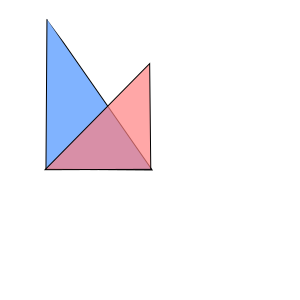
\includegraphics[width=5cm]{place_figure_probleme_point}\\
    \emph{Ici, une arête coïncidente a bien été trouvée mais il n'y a pas la place pour que la pièce se place dans le modèle. Cette pièce peut alors soit être en dehors du modèle initial, soit sur une autre pièce (puisque notre méthode est récursive et que le modèle dans ce cas est une étape).}\\
    \end{center}

    Pour résoudre ce problème, un algorithme existant et assez complexe a été utilisé. Pour chaque sommet de la figure, le nombre d'arêtes ayant un point à la même hauteur que le sommet est compté. Dans le cas où un nombre impair de points de chaque coté de l'arête est trouvé, alors le point est à l'intérieur du modèle. Sinon, il se trouve à l'extérieur.\\
    La source de l'algorithme est disponible à l'adresse suivante : \emph{http://alienryderflex.com/polygon/}\\ 

    Après avoir testé l'ensemble des points de la pièce positionnée et ainsi que l'ensemble des points de son symétrique par rapport à l'arête de la base, l'une des pièces est identifiée comme étant en partie à l'extérieur du modèle.\\ \ \\

    L'algorithme chargé de générer l'ensemble des placements possibles va donc pour une pièce et un modèle donnés, tenter de trouver les positions disponibles. Pour cela, la première méthode va être utilisée puis de la seconde. Dans le deux cas, la validité des résultats trouvés est vérifiée.\\
    Dans le cas où aucun placement n'est possible (c'est à dire si le modèle est trop petit pour accueillir la pièce ou si aucun angle ni aucune arête ne convient), l'algorithme échoue.
	
		\section{Soustraction d'une forme au modèle}
		
		Le second problème mathématique que la résolution exigeait de résoudre est la soustraction d'une forme au modèle. En effet, la solution la plus simple résidait dans le fait de placer une forme dans le modèle pour ensuite renvoyer un nouveau problème et recommencer le casse-t\^ete la forme placée en moins avec le nouveau modèle.\\
		Ce problème imposait donc plusieurs sous-étapes pour pouvoir retourner de façon efficace le nouveau modèle. Ces sous-étapes sont la découverte des tous les points du nouveau modèle, puis la suppression d'éventuels points qui seraient inutiles. Une précision importante à apporter est le fait qu'il faut conserver l'ordre des points du modèle afin de conserver la forme voulue. Le travail nécessite donc de passer non pas seulement par des points mais par des arêtes.\\
		Le fait d'utiliser des arêtes a permis de réunir les deux sous-étapes puisque la suppression de points superflus se fait tout au long de la découverte des nouveaux points. Malgré tout, plusieurs étapes sont nécessaire pour la découverte du nouveau modèle.\\ \ \\
		La première étape, tout comme lors de l'étape du placement d'une pièce, est de trouver une arête commune à la pièce et au modèle. La différence étant qu'ici, l'algorithme est sûr de trouver au moins une arête commune. Dans le cas où plusieurs arêtes correspondent, l'algorithme prend simplement la première qui arrive puisque le choix de l'arête n'a pas d'importance.\\
		Un fois cette arête commune choisie, on doit vérifier si le sens de la forme est la même que le sens du modèle. En effet, lors de la recherche d'une arête commune, on cherche sans distinction si l'arête est présentée dans le même sens ou non. Par exemple, si sur la forme l'arête a pour coordonnées $(0,100)$ et sur le modèle les coordonnées $(100,0)$, il faut "retourner" les arêtes afin que les coordonnées correspondent.\\
		Une fois la pièce à insérer mise en bonne forme, ses arêtes sont ajoutées sans test dans le modèle juste après l'arête commune entre la pièce et la forme. Ainsi, les arêtes de la pièces cont ajoutées au bon endroit dans le modèle.\\
		
		\begin{center}
			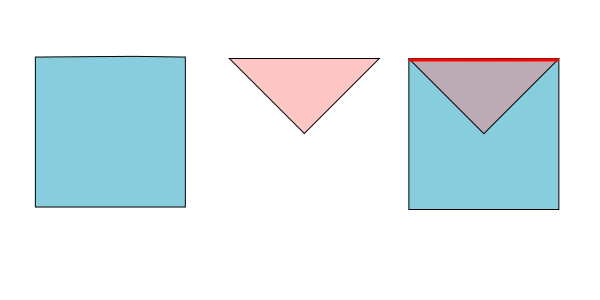
\includegraphics[width=12cm]{soustraction_arete_1}\\
			\emph{Ici, on peut voir que l'arête du haut du carré est commune au triangle placé. On va donc placer les arêtes du triangle juste après l'arête du modèle qui est commune à celle du triangle. Comme le triangle possède aussi cette arête, le placement est correct.\\}
		\end{center}
		
		Cependant, une fois cette étape effectuée, on est en présence de doublons d'arêtes dans notre nouveau modèle. Cette nouvelle étape va donc vérifier les arêtes en double (quel que soit le sens). Ces dernières sont éliminées du modèle. Aucune occurrence de ces arêtes ne doit rester dans le nouveau modèle. En effet, en faisant apparaître des arêtes en double, l'algorithme indique que ce sont des arêtes qui étaient communes et qui n'ont donc plus lieu d'être du fait de la soustraction de la pièce.\\
		
		\begin{center}
			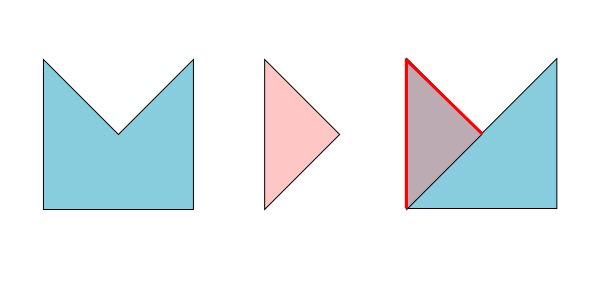
\includegraphics[width=12cm]{soustraction_arete_2}\\
			\emph{Dans ce cas, on voit que deux arêtes sont communes. La partie de l'algorithme recherchant les doublons d'arêtes va donc supprimer les occurrences de ces arêtes, ici surlignées en rouge. Le point en haut à gauche de l'ancien carré est donc supprimé automatiquement et le nouveau modèle adopte la bonne forme.}
		\end{center}
		
		
		Comme le travail est fait sous forme de points, l'algorithme fait repasser ensuite chaque arête en point et vérifie alors par prévention si aucun point n'apparaît en double à la suite. Si c'est le cas, on supprime une occurrence de ce point. \\
		Enfin, comme l'algorithme a utilisé les arêtes, la première et la dernière arête ont un point en commun. Ce point va donc être présent au début et à la fin de la liste des points du nouveau modèle. Il faut donc supprimer celui qui se situe à la fin.\\ \ \\
		
		L'algorithme gère naturellement le cas d'arrêt de ce problème puisque lorsque le modèle passé correspond à la pièce, il va retourner un ensemble de points vides.
		
		\section{Implémentation de l'algorithme DFS (profondeur d'abord)}
		
 			\subsection{Analyse de la recherche}

		Le Tangram est un jeu qui n'est pas représentable par un système de coût suivant le placement de chaque pièce. En effet, toutes les pièces devant être placées, il n'y a pas de concurrence directe entre ces pièces. Même s'il était possible de mettre en place ce système de coût, il ne serait pas pertinent de le
faire car les scores de chaque pièce seraient égaux.\\
		Ici, le problème peut se modéliser par un arbre de recherche qui est cependant assez complexe. De très nombreuses configurations sont possibles pour chaque nœud. L'exemple du carré ci-dessous permet d'indiquer comment se construit l'arbre de recherche. Les étapes sont pour la résolution:
		\begin{itemize}
			\item Sélection de la première pièce: un gros triangle;
			\item Celui-ci est positionnable sur le dessin mais à plusieurs endroits;
			\item Ainsi, en plus d'avoir comme première branche le gros triangle, les branches filles représentent chaque configuration possible du gros triangle;
			\item Pour chacune de ses branches, on essaye avec les pièces restantes, qui elles-même possèdent en sous-branche à nouveau leurs différentes configurations.\\
		\end{itemize}
		
		Ainsi, chaque profondeur est alternée par le choix d'une pièce puis d'une de ses différentes configurations. Si une pièce ne possède aucun placement disponible, elle apparaît tout de même dans l'arbre mais n'a aucun enfant. S'il est considéré qu'un niveau est constitué de deux profondeurs, c'est à dire d'une pièce ainsi que de ses configurations, une solution est trouvée lorsque la recherche atteint le niveau 7, correspondant au nombre de pièces composant le
jeu du Tangram.

			\subsection{Choix de la recherche}

		Dans la recherche à effectuer, il est donc nécessaire de parcourir chaque branche jusqu'à sa fin. Dans de nombreux cas, plusieurs solutions sont possibles, m\^eme si elles sont souvent proches (elles diffèrent pas rotation par exemple). Cependant, une seule solution étant nécessaire, il est plus pertinent de se diriger le plus rapidement vers la fin de chaque branche. Il faut donc exclure l'idée d'utiliser un algorithme parcourant en largeur l'arbre à construire et plutôt se focaliser sur une recherche en profondeur.\\
		L'algorithme DFS (Depth First Search) est donc retenu. Il convient parfaitement à la situation puisqu'il étend le nœud du graphe et ses successeurs le plus longtemps possible jusqu'à atteindre le nœud but, ou jusqu'à atteindre un nœud
n'ayant plus de fils. Dans ce cas, l'algorithme effectue du "backtracking" et permet d'explorer les branches suivantes. \\
		Si la recherche atteint un nœud but (c'est à dire que toutes les pièces ont pu être placées avec succès), on arrête la recherche puisqu'on a résolu le problème. Chercher une autre solution ne ferait que surcharger le programme.


	\newpage
	
	\chapter{Représentation informatique du problème}
	
	Le passage de la phase d'analyse à la phase "informatique" du pour la résolution du tangram s'avère beaucoup plus complexe que ce qui avait été prévu. Cependant, des représentations précises ont été adoptées. Ces représentations se traduisent par des structures de données fixes qui ont été mises en place afin de mieux coordonner les différents prédicats Prolog.

	    \section{Structures de données}

        La structure majeure qui a dû être mise en place lors de l'implémentation du projet se doit de permettre la définition des pièces du Tangram ainsi que des différentes patterns.\\ \ \\ 
        
        Après avoir envisagé plusieurs solutions il a été décidé de représenter toutes les figures dans un repère orthonormé où chaque point d'une figure est représenté par deux coordonnées X et Y. \\
        En ce qui concerne Prolog, un point est donc représenté par une liste de deux éléments où le premier est la coordonnée en abscisse (X) et le second celle en ordonnée (Y).\\
		Comme en géométrie où une figure est définie par un ensemble de points, en Prolog, la représentation des figures se structure selon une liste de points, ces derniers étant ordonnés de façon à ce que deux points l'un à coté de l'autre dans la liste forment une arête sur la figure. Plus simplement, les points sont placés dans l'ordre. Bien entendu, le couple formé par le premier et le dernier point représente également une arête.\\
		Les pièces sont donc représentées par des listes de points, chacune de ces pièces ayant un point qui est positionné à l'origine du repère. Grâce à cette modélisation, lors du placement des pièces sur un modèle, il suffira de transformer la figure par rotation ou par translation vers sa position.\\
		Les modèles sont un peu plus complexes à modéliser car ils peuvent être divisés en plusieurs parties pour certaines configurations. Aussi, comme il n'est pas possible de prévoir la position des pièces à l'avance, il se peut que le positionnement d'une pièce dans le modèle forme deux nouveaux sous modèles. Il a donc été choisi de modéliser un modèle suivant une liste de figures. 


        \begin{center}
            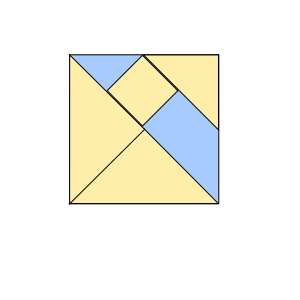
\includegraphics[width=5cm]{representation_sousfigure}\\
            \emph{Dans le cas ci-dessus, on remarque que le placement du carré dans le modèle fait passer celui-ci d'une partie à deux en sortie de l'algorithme de soustraction d'une pièce à un modèle.}
        \end{center}
        
        
        \subsection{Espace d'états}

		Les états sont composés de plusieurs éléments :
		\begin{itemize}
			\item les pièces restantes à placer;
			\item les coordonnées représentant le modèle restant à combler;
			\item les pièces déjà placées, ainsi que leurs coordonnées.
		\end{itemize}

		Il est donc possible de coder ces états comme suit:\\
		$(Pieces, Modele, PiecesPlacees)$\\

		$Pieces$ est défini dans l'ensemble des pièces disponibles pour résoudre le Tangram (soit 7 pièces, donc 7 valeurs différentes).\\
		$PiecesPlacees$ est défini de manière semblable, sauf que les coordonnées sont définies dans le plan défini par le modèle.\\
		$Modele$ est défini également dans le plan, ses valeurs ne
pouvant aussi pas être plus petite ou plus grande que les différentes coordonnées composant le modèle de base. Il est important de noter que toutes les coordonnées sont positives (définies dans la partie Nord-Est du repère).\\ \ \\

		\paragraph{Exemple pour les coordonnées pour le modèle du carré\\}
 
		Les coordonnées sont définies telles que $0\ \leq\ X\ \leq\ 100$ et $0\ \leq\ Y\ \leq\ 100$.\\ \ \\

		\paragraph{Exemple de différents états\\}

		État initial pour le modèle du carré:\\
\begin{verbatim}
(
	(petit_triangle, gros_triangle, moyen_triangle, carre,	
		parallelogramme, petit_triangle, gros_triangle),
	((0, 0), (100, 0), (100, 100), (0, 100)),						
	()														
)
\end{verbatim}


État intermédiaire:\\
\begin{verbatim}
(
	(petit_triangle, moyen_triangle, carre,					
		parallelogramme, petit_triangle), 
	((100, 0), (100, 100), (0, 100)),							   
	(														
		(gros_triangle, 
			((0, 0), (0, 100), (50, 50))
		),
		(gros_triangle, 
			((0, 0), (100, 0), (50, 50))
		)
	)
)
\end{verbatim}


État final:\\
\begin{verbatim}
(
	(),														
	(),														
	(													   
		(gros_triangle,
			((0, 0), (0, 100), (50, 50))
		),
		(gros_triangle, 
			((0, 0), (100, 0), (50, 50))
		),
		...,
		(moyen_triangle,
			((100, 50), (100, 100), (50, 100))
		)
	)
)
\end{verbatim}

			\subsection{Système de production}

		Les règles du système de production traitent des contraintes que les pièces placées doivent respecter, mais ne rentrent pas dans le déroulement de la recherche de placement des pièces. Il est très difficile pour un problème de ce type de définir un ensemble de règles précises, puisque celles-ci diffèrent en fonction du modèle à résoudre.\\
		Les règles concernant les ensembles de définition des coordonnées sont les premières à être affectées par ce problème. Ainsi il convient d'adapter à chaque cas ces règles. De plus, le modèle évoluant constamment, il n'est pas possible de définir ces règles, car elles vont évoluer en même temps que le modèle. \\
Une règle simple $(R0)$ pour ceci peut être que chaque point d'une pièce dans $PiecesPlacees$ à un état $N$ doit
être dans la surface de $Modele$ à un état $N-1$.\\

Les autres règles, plus simples à définir, sont:
	\begin{itemize}
		\item $(R1)$ Le nombre de pièces dans $Pieces$ est compris entre 0 et 7;
		\item $(R2)$ Le nombre de pièces dans $PiecesPlacees$ est compris entre 0 et 7;
		\item $(R3)$ L'aire du $Modele$ à un état $N$ doit être égal à l'aire du $Modele$ à l'état $N-1$ moins l'aire de la dernière pièce dans $PiecesPlacees$;\\
		Remarque: cette règle n'a pas été développée mais pourrait l'être à l'avenir.
		\item $(R4)$ $Modele$ est vide si $Pieces$ est vide et que le nombre de pièces dans $PiecesPlacees$
est égal à 7;
		\item $(R5)$ Le nombre de pièces est égal à 7 moins le nombre de pièces dans $PiecesPlacees$;
		\item $(R6)$ Le nombre de pièces dans $PiecesPlacees$ est égal à 7 moins le nombre de pièces dans $Pieces$.
	\end{itemize}
	
	\chapter{Résultats obtenus et exemples}
	
	De nombreux problèmes ayant été rencontrés durant le projet, les résultats obtenus n'indiquent pas une résolution totale de différents modèles. Ceci est d\^u au fait des différentes difficultés apparues sur les algorithmes mathématiques touchant à la géométrie.\\
	Malgré tout, sur des modèles simples, l'ensemble des prédicats fonctionnent ensemble et parviennent à s'articuler pour fournir des résultats. Le logiciel et donc fonctionnel dans son ensemble.\\ \ \\
	
	Les deux Tangrams suivants sont résolus sans problèmes par le logiciel et sont issus du modèle carré classique connu de tous:
	\begin{itemize}
		\item Cas du demi carré avec deux triangles à place:
		\begin{center}
			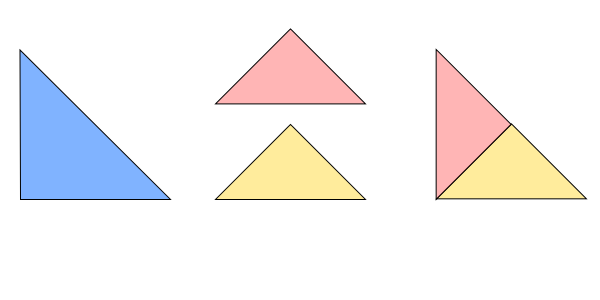
\includegraphics[width=12cm]{resultat_1}\\
		\end{center}
		\item Cas plus complexe avec trois triangles à placer:
		\begin{center}
			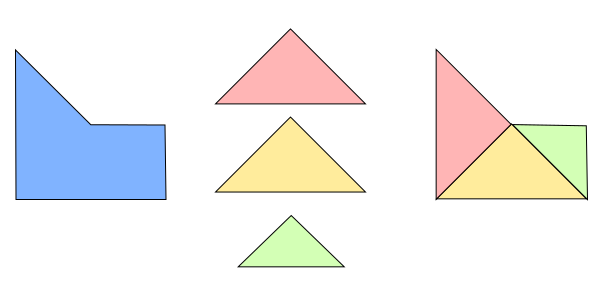
\includegraphics[width=12cm]{resultat_2}
		\end{center}
	\end{itemize}
	
	\chapter{Problèmes rencontrés}
	
	Comme déjà abordé tout au long de ce rapport, de nombreux problèmes ont été rencontrés lors du projet. La première des difficultés était que le problème n'a que très peu été traité jusqu'à aujourd'hui et qu'il fallait donc partir de zéro au niveau des idées de conception de l'IA.\\
	Des sous-problèmes ont donc rapidement été isolés, cependant, c'est pendant la résolution de ces différents problèmes que les plus grosses difficultés ont été rencontrées, notamment pour les parties mathématiques.\\
	Ces difficultés ont été assez rapidement surmontées algorithmiquement, mais lors du passage en Prolog, de nouvelles difficultés ont été rencontrées. En effet, la formalisation de problèmes géométriques dans ce langage ne nous a pas apparu aisé. Il reste donc à ce jour certains cas où les prédicats liés à la géométrie (particulièrement pour le placement) qui ne fonctionnent pas. Ceci est dû au fait que de nombreux différents cas étaient à gérer dont de nombreux qui étaient isolés. Ces cas là n'ont donc pas tous été traités, soit parce qu'ils n'ont pas été découverts, soit parce qu'aucune solution n'a été trouvée.\\
	Du fait de ces difficultés, une interface graphique n'a pas pu être développée par manque de temps. Les résultats sont donc retournés en ligne de commande ce qui n'empêche pas le bon fonctionnement du programme.
	
	\chapter{Améliorations possibles}
	
	Comme le programme n'est pas en mesure de gérer tous les cas, de nombreuses améliorations pourraient encore \^etre apportées, en particulier pour la gestion des nombreux cas particuliers. Aussi, comme il en a été question plus t\^ot dans ce rapport, la vérification par l'aire, c'est-à-dire en comparant l'aire du modèle avec la somme des aires des figures restant à \^etre placées, nous paraissait une méthode intéressante à implémenter. Ceci éviterait de descendre dans des branches vouées à l’échec lors de l'exécution de l'algorithme de recherche d'une solution.
	
	\chapter*{Conclusion}
	\addcontentsline{toc}{chapter}{Conclusion}
	
	
	
	
		
	\newpage	
		
	\tableofcontents

	\begin{appendices}

    \chapter{Prédicat soustraction}
    \begin{verbatim}
    % file : soustraction.pl
    soustraction([Patterns], Piece, [NewPatterns]):-

    tools:liste_all_couple_aretes(Patterns,CoupleAretePatterns),
    tools:liste_all_couple_aretes(Piece,CoupleAretePiece),

    search_commmon_arete(CoupleAretePatterns,CoupleAretePiece,Arete),
    search_sens_forme(CoupleAretePiece,Arete,Sens),
    retourne_forme(CoupleAretePiece,Sens,CoupleAretePiece1),

    mix_pattern_forme(CoupleAretePatterns,CoupleAretePiece1,Arete,Mixed),
    clean_double_arete(Mixed,CleanedMixed),

    arete_to_point(CleanedMixed,NewListPoint),
    clean_double_point(NewListPoint,NewPatterns1),
    clean_first_last_double_point(NewPatterns1,NewPatterns).
    \end{verbatim}

    \begin{itemize}
        \item \textbf{Patterns} : variable représentant le modèle actuel à réaliser;
        \item \textbf{Piece} : variable représentant la pièce positionné en fonction du modèle;
        \item \textbf{NewPatterns} : variable représentant le nouveau modèle.
    \end{itemize}

\chapter{Prédicat placePiece}
    \begin{verbatim}

% file : placePiece.pl
placePiece(Piece,Patterns,ReturnPiece):-
    test_placement_patterns_exact_match(Piece,Patterns,Placement),
    positionne(Piece,Placement,NewPiece),
    test_all_placement(NewPiece,Patterns,Placement,ReturnPiece).

placePiece(Piece,Patterns,ReturnPiece):-
    test_placement_patterns_angle_match(Piece,Patterns,Placement),
    positionne(Piece,Placement,[Axe1,Axe2],NewPiece),
    test_placement(NewPiece,Patterns,[Axe1,Axe2],ReturnPiece).

    \end{verbatim}

    \begin{itemize}
        \item \textbf{Piece} : variable représentant la pièce à placer;
        \item \textbf{Patterns} : variable représentant le modèle où placer la pièce;
        \item \textbf{ReturnPiece} : variable représentant la pièce correctement placée.
    \end{itemize}


	\chapter{Prédicat essai\_piece}
	
    \begin{verbatim}

% file : main.pl
essai_piece(_,[[]],_,_):-!.
essai_piece([], _, _, _) :- !.
essai_piece(_, [], Solution, _) :- !, 
    affiche_resultat(Solution).

essai_piece(_, _, _, 0) :- 
    write_ln('\tBout de la branche atteint'), !, fail.

essai_piece([Piece|PiecesRestantes], Pattern, [[Piece, Placements]|PiecesRetenues], _) :-
    points_piece(Piece, PointsPiece),
    write('Essai de la pièce '),
    write(Piece),
    placePiece(PointsPiece, Pattern, Placements),
    retirer_piece(PiecesRestantes, Pattern, Placements, PiecesRetenues).

essai_piece([PieceNonUtilisee|PiecesRestantes], Pattern, PiecesRetenues, N) :- 
    append(PiecesRestantes, [PieceNonUtilisee], Pieces), N1 is N-1,
    write_ln(' -> la pièce est mise de côté pour le moment'),
    essai_piece(Pieces, Pattern, PiecesRetenues, N1).  
    
    \end{verbatim}

    \begin{itemize}
        \item \textbf{ListePiece} : variable représentant la liste des pièces à placer;
        \item \textbf{Pattern} : variable représentant le modèle à réaliser;
        \item \textbf{PiecesRetenues} : variable représentant la liste des pièces placées;
        \item \textbf{N} : variable représentant la profondeur maximale de l'arbre de réalisation.
    \end{itemize}


\end{appendices} 




		
\end{document}




